

Along with the work of the two adder designs, a brief survey about dynamic logic has been made. The main issue is to find whether there are new dynamic logic technologies that can be used in adders, instead of the standard static MOS structures. The main characteristics of dynamic logic are introduced and discussed, in order to understand the positive and negative aspects of this design technique. For further general information \cite{Rabaey} can be seen.

\section{General aspects}

\paragraph{} Dynamic logic is an alternative design approach of Pseudo NMOS and static CMOS and presents several advantages similar to these ones. Figure \ref{fig:dynamic} shows the general schematic of a dynamic logic topology. In this case a pull down network is used, just like the static CMOS logic, but the dual pull up network can be used instead.

\begin{figure}[H]
\centering
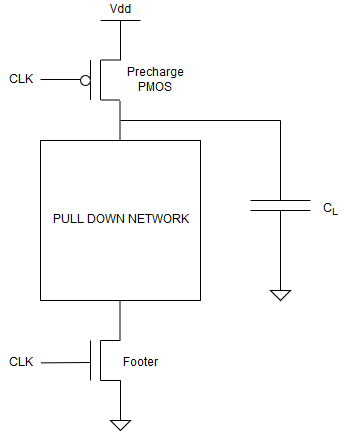
\includegraphics[width = 7 cm]{dinamic_logic_survey/Dynamic_logic-Page-1.png}
\caption{Dynamic logic general schematic.}
\label{fig:dynamic}
\end{figure}

\paragraph{} The first positive feature is the lower area occupation: the number of transistors increases linearly with the number of inputs. A generic dynamic N port gate has N+2 transistors, which is close to the pseudo NMOS design, and less than the static CMOS logic, which is 2N. The first N transistors are needed to implement the Pull Down (or Up) Network, while a PMOS and NMOS are used for the clock signal. The clock signal is needed to define the two working phases of the circuit, the pre-charge and the evaluation phases.

\paragraph{} Another important aspect is the absence of static power consumption, unlike pseudo NMOS but similar to the static CMOS logic. The static power is the generated power due to short path between supply voltage and ground.

\paragraph{} Furthermore, the circuit presents a lower fan-in with respect to the static CMOS implementation, and this aspect leads dynamic logic to better performance. These features together makes dynamic logic suitable for high performance and low cost implementation.

\paragraph{} The dynamic logic presents several drawbacks, though. The need of a clock signal affects negatively power consumption, since at least two transistors are charged and discharged in each clock cycle. Power consumption is also affected by an activity factor $\alpha_{1 \rightarrow 0}$ higher than the static CMOS. For example, if all the inputs of a NOR gate have a uniform statistic distribution, the activity factor of the dynamic logic and static logic implementations are, respectively the (\ref{alpha_dynamic}) and (\ref{alpha_static}):
\begin{equation}
\alpha_{dynamic} = 75\% \
\label{alpha_dynamic}
\end{equation}
\begin{equation}
\alpha_{static} = 18,75\%
\label{alpha_static}
\end{equation}
The dynamic power consumption is given by the (\ref{dynamic_power_consumption}):
\begin{equation}
P_{dyn} = \alpha\cdot C_L V_{dd}^2 f_{clk}
\label{dynamic_power_consumption}
\end{equation}
which is proportional to the activity factor. Leakage currents are to be considered also, since they can discharge the output node, and determine the minimum period between two pre-charge phases, which is the minimum clock frequency accepted. This value is about some KHz. Leakage currents tend to discharge the output node, since this one is an high impedance node. This problem can be resolved by using a \textit{bleeder} transistor \cite{Rabaey}.

\paragraph{} Another aspect to be considered is the charge sharing with other output and with the clock signal (\textit{clock feedthrough}) which affects dramatically reliability. The latter can forward bias the drain-bulk junction of the pre-charge MOS  which  can switch the high impedance node voltage from '1' to '0' or, worse, cause \textit{latch-up}.

\newpage
\section{Domino design techniques}
An evolution of dynamic logic is the Domino one, which was first described by \cite{Krambeck}. Figure \ref{fig:DOMINO} shows the schematic of a single stage Domino circuit.

\begin{figure}[H]
\centering
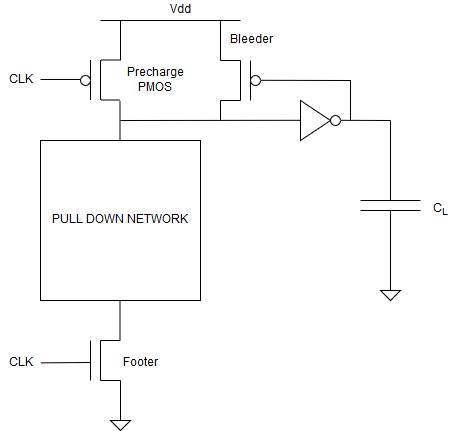
\includegraphics[width = 7 cm]{dinamic_logic_survey/Dynamic_logic-Page-2.png}
\caption{General schematic of domino logic circuit. The bleeder transistor is optional but highly recommended, in order to avoid information loss due to leakage currents.}
\label{fig:DOMINO}
\end{figure}

The main advantage is that Domino circuits can be placed in multiple stages with the same topology and can be pipelined with multiphase clocking system \cite{Verma} instead of using latches. At architectural level, the adoption of multiphase clocking prevent the use  High performance are reached at the expense of higher power consumption due to the more clock lines needed.


\section{Dual Rail Domino Logic}
A particularly and interisting case of Domino logic is the Dual Rail Domino Logic (DRDL) implementation in order to make low power adders \cite{dominoAdder8}. An example of Dual rail Domino circuit is reported in figure \ref{fig:Dual Rail}.
\begin{figure}[H]
\centering
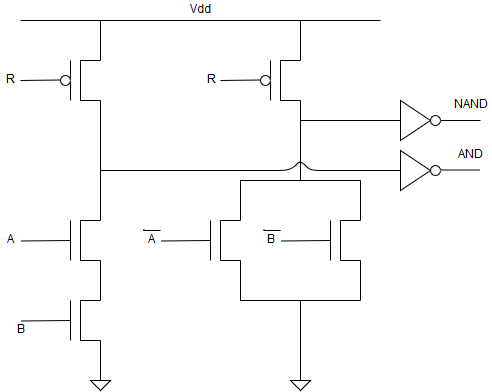
\includegraphics[width = 7 cm]{dinamic_logic_survey/Dynamic_logic-Page-3.png}
\caption{Dual Rail Domino logic implementation of a NAND circuit. The main advantage is to have inverting and non inverting function, at the expense of more area occupation.}
\label{fig:Dual Rail} 
\end{figure}
In this implementation, circuit works in near threshold in order to reduce power consumption and uses an asynchronous pipeline. This approach reduces the energy-delay product, defined as:
\begin{equation}
EDP = E_{op} \times \tau_{delay}
\end{equation}
where $E_{op}$ is the energy drained by the device during the SPICE simulation and $\tau_{delay}$. Although there is an improvement in energy consumption, performance and area become worse than a synchronous pipelined static CMOS implementation. Energy consumption, number of transistors and delay of \cite{dominoAdder8} are reported in table \ref{tab:8bitAdder}. The worst case is used for synchronous adder and average case for the dual rail Domino logic one.
\begin{table}[H]
\centering
\begin{tabular}{|c|c|c|c|}
\hline 
 & Transistors & Delay $\mu s$ & Energy $fJ$ \\ 
\hline 
DRDL & 1460 & 62.6 & 499 \\ 
\hline 
CMOS & 764 & 59.3 & 871 \\ 
\hline 
\end{tabular}
\caption{Comparison between DRDL and static CMOS 8-bit adder.}
\label{tab:8bitAdder}
\end{table}
As it can be seen, energy consumption is improved with respect to CMOS at the cost of almost double area and a little worse delay.


\section{Technology scaling comparison}
An important issue is to find whether technology scaling improve significantly the Domino circuits power consumption with respect to static CMOS logic. Two interesting works are found are compared in table .
\begin{table}[H]
\centering
\begin{tabular}{|c|c|c|c|}
\hline 
 & Power & Pwr diff. with the previous gate \\ 
\hline 
32 nm FinFET static NAND2 in \cite{Nalamwar} & 440 nW & 0 \% \\ 
\hline 
25 nm FinFET Domino AND2 in \cite{Rasouli} & 1.6 $\mu W$ & +264 \% \\
\hline 
32 nm FinFET static NOR2 \cite{Nalamwar} & 440 nW & 0 \% \\ 
\hline 
25 nm FinFET Domino OR2 \cite{Rasouli} & 4 $\mu W$ & +810 \% \\ 
\hline 
\end{tabular} 
\end{table}
Despite of the use of a better technology, the Domino logic suffers for higher power consumption, compared with the static CMOS logic.

\section{Final Considerations}
Dynamic logic based circuits are a good alternative if area and performance are critical aspects of the design. Multistage Domino circuits can be also pipelined with a multiphase clock approach, so no more latches are needed and there is more area saving. These aspects are  balanced by a higher power consumption, which can be far higher than the static logic. Scaling does not improve the power consumption issue, so dynamic logic is generally not suitable for low power implementations, which is the current tendency. The Dual Rail Domino logic can be an interesting choice in case of asynchronous pipeline designs, since energy consumption is better than synchronous static implementations, although they occupy more area and have a performance similar to the static logic.